\documentclass[senior]{IPSstyle}

  \Year{2018}
  \Month{July}
  \Author{44161643-2: HOU BOWEI}

  \Title{Without Wearing Device Gaze Estimation from Image}

  \Advisor{Professor Yoshie}

\usepackage{amssymb,amsmath}

\usepackage{mathptmx}
\usepackage{helvet}
\usepackage{courier}
\usepackage{type1cm}

\usepackage{makeidx}
\usepackage{graphicx,subfigure}
\usepackage{multicol}
\usepackage{multirow}
\usepackage[bottom]{footmisc}

\usepackage{mathrsfs}
\usepackage{amssymb,amsmath}
\usepackage{amsfonts}
\usepackage{color}
\usepackage{CJKutf8}

\usepackage{listings}
\usepackage{algorithm,algorithmicx,algpseudocode}
\usepackage[toc,page,title,titletoc,header]{appendix}

\renewcommand{\algorithmicrequire}{\textbf{Input:}}
\renewcommand{\algorithmicensure}{\textbf{Output:}}

\Abstract{
Gaze estimation is a hot and traditional area in both computer vision and interaction. In the 90s, gaze estimation was developed by physics scientists, and the main usage is in the medicine surgery area. In that era, gaze estimation needs a lot of equipment on the head and a laboratory with lots of sensors. As the time moving on, the equipment is becoming smaller and the number of sensors are becoming lesser. However, we still need calibration device or eye-tracker facilities. 
Normally, a gaze estimation method is one kind of pipe line. They will use sensors to extract parameters of the environment. Such as illumination, position of the camera and the distance between the person and camera. After that, eye detector device is applied to take picture near your eyes and then get the shape of the eyeball. Finally, all the data extracted from the equipment, which as the landmarks of the head and eyes, will be fixed into a physical model of human’s head, with the predefined math equation eye direction can be calculated.
Here comes up a purpose, why don’t we use images only to detect the gaze direction. Inspired by the potential power of convolutional neural network which is proved to be good at extract information from image, it will be a convenient way to make an end-to-end algorithm based on specific neural network.
}

\Keywords{Convolutional Networks, Gaze Estimation, Deep Learning, Computer Vision, Eye Gaze}

\Acknowledgments{
I came to Japan almost two years ago without any experience of Japanese. Japan is new to me, but the Japanese are so nice that they make me feel at home. 

I really appreciate the first year learning lessons in IPS, teachers help me to base the fundamental knowledge of data science, like the NLP concerning class, Computer Vision concerning class digital signal processing, and machine learning concerned pattern recognition.

The laboratory is another place where I really admire to live in. Professor Yoshie helped us with supporting very powerful server to do experiments. Also we have a very comfortable enviorment in the lab. 

At last, I want to pay appreciation to my fellows, all the students in the lab. We study together and solve problems together, during the two-years learning process, not only knowledge but also friendship is developed. The memory of being together will reminds all my life long.
}


\begin{document}

 \makepreliminarypages
 \singlespace
 \frontmatter
 \tableofcontents
 \listoffigures
 \listoftables
 \mainmatter
 \clearemptydoublepage
 \setlength{\baselineskip}{23.0pt}

\chapter{Introduction} \label{introduction}



\section{Background}

\begin{figure}[t]
  \centering
  % Requires \usepackage{graphicx}
  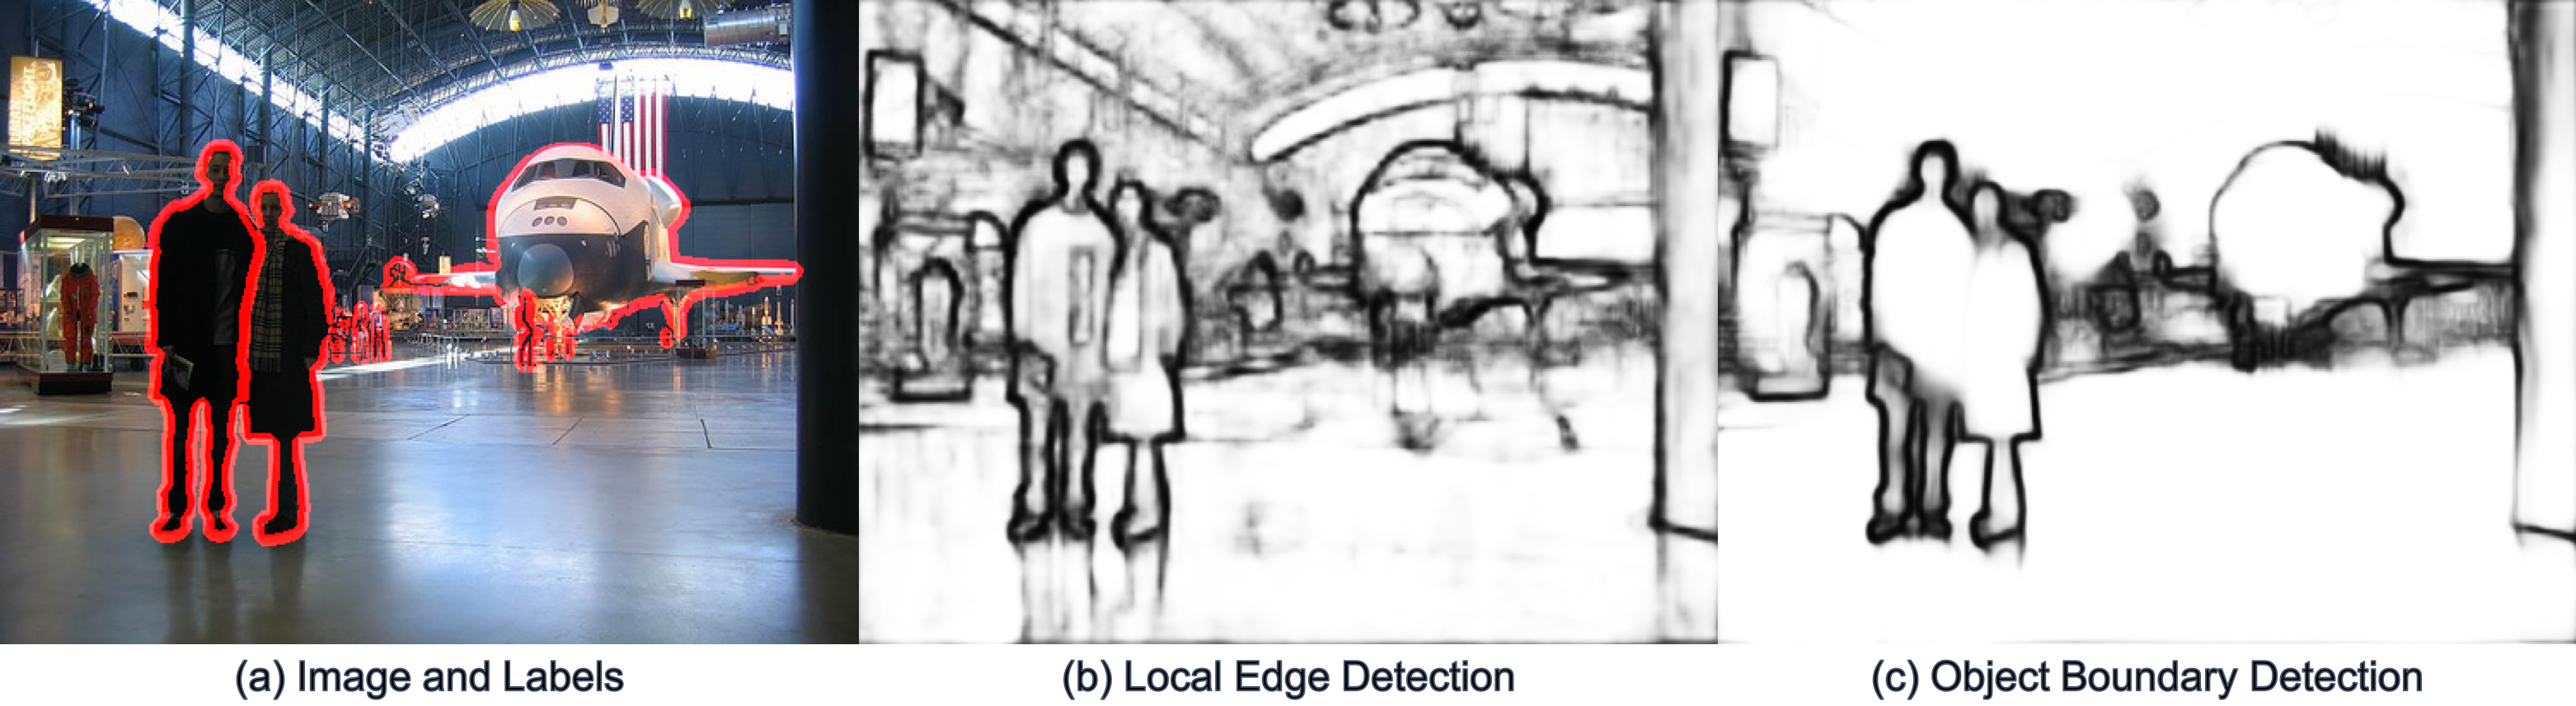
\includegraphics[width=15cm]{object_boundary_vs_local_edge.png}\\
  \caption{Object-level boundary detection is different from the traditional local edge detection, where the former mainly focuses on detecting the high-level semantic boundaries. The first image contains the annotations, which are marked with red lines, for object-level boundary detection.}\label{object_boundary_vs_local_edge}
\end{figure}
% 
Gaze estimation is a traditional area in computer vision and computer interaction. Since long time ago, finding the gaze direction is the object in medical and facial analyze projects. In the ancient times, such kind of technologies are based on heavy equipment, including electro-occulography and coil embed lens. When it comes to video eye gaze studying, the first one is concerned with airplane pilot, mainly for flight control systems in 1940s\cite{mohamed2007history}.

%%%%%%%%%%%%%%%%%%%%%%%%%%%%%%%%%%%%%%%%%%%%%%%%%%%%%%%%%%%%%%%%%%%%%%%%%%%%%%%


\section{Application Scenes}

\subsection{Special Device to Check Pupil}

\subsection{Car Industry Detect Eye Movement}

\subsection{Play Station}

%%%%%%%%%%%%%%%%%%%%%%%%%%%%%%%%%%%%%%%%%%%%%%%%%%%%%%%%%%%%%%%%%%%%%%%%%%%%%%%


\section{Organization of the thesis}

%%%%%%%%%%%%%%%%%%%%%%%%%%%%%%%%%%%%%%%%%%%%%%%%%%%%%%%%%%%%%%Chapter 3
\chapter{Related Work} \label{related_work}
%%%%%%%%%%%%%%%%%%%%%%%%%%%%%%%%%%%%%%%%%%%%%%%%%%%%%%%%%%%%%%Chapter 3


%%%%%%%%%%%%%%%%%%%%%%%%%%%%%%%%%%%%%%%%%%%%%%%%%%%%%%%%%%%%%%%%%%%%%%%%%%%%%%%



\section{Traditional gaze estimation}
\subsection{Homograph}
\subsection{3D Re-projection}
\subsection{Deep learning based methods}

\section{Object Boundary Detection in Natural Images}

%%%%%%%%%%%%%%%%%%%%%%%%%%%%%%%%%%%%%%%%%%%%%%%%%%%%%%%%%%%%%%%%%%%%%%%%%%%%%%%


\chapter{Purpose} \label{methodology}

\section{Original Pipeline}
\subsection{Traditional Pipeline Algorithm}


%%%%%%%%%%%%%%%%%%%%%%%%%%%%%%%%%%%%%%%%%%%%%%%%%%%%%%%%%%%%%%%%%%%%%%%%%%%%%%%
\section{Network Structure} \label{network structure}
\section{Training Phase} \label{training phase}
\subsection{Formulation of the Multi-recursive-input}


\subsection{Loss Function}



\section{Testing Phase} \label{testing phase}


\section{Model Interpretation} \label{interpretation}
\subsection{Cascaded Architecture \emph{vs.} Single-stage Architecture}

\subsection{Multi-recursive-input \emph{vs.} Single-recursive-input}


\subsection{End-to-end Training \emph{vs.} Stepwise Self-tuning}

%%%%%%%%%%%%%%%%%%%%%%%%%%%%%%%%%%%%%%%%%%%%%%%%%%%%%%%%%%%%%%%%%%%%%%%%%%%%%%%


\chapter{Experiments} \label{experiments}


\section{Neuronal Boundary Detection in EM Images}



\subsection{Evaluation Metric}

\subsection{Mouse Piriform Cortex Dataset}\label{experiment of piriform}


\subsection{ISBI 2012 EM Segmentation Dataset}


\section{Object Boundary Detection in Natural Images}
\subsection{Metrics}
\subsection{PASCAL VOC Contour Dataset}

\section{Control Experiments for Model Interpretation}3

\subsection{Evaluations on Cascaded Architecture \emph{vs.} Single-stage Architecture}

\subsection{Evaluations on Multi-recursive-input vs. Single-recursive-input}

\subsection{Evaluations on End-to-end Training vs. Stepwise Self-tuning}


\bibliographystyle{IEEEtran}
\bibliography{LUOreference}
\end{document}
